\documentclass[a4paper,12pt]{article}
\usepackage[a4paper,top=1.3cm,bottom=2cm,left=1.5cm,right=1.5cm,marginparwidth=0.75cm]{geometry}
\usepackage{setspace}
\usepackage{cmap}
\usepackage{mathtext}
\usepackage[T2A]{fontenc}
\usepackage[utf8]{inputenc}
\usepackage[english,russian]{babel}
\usepackage{multirow}
\usepackage{graphicx}
\usepackage{wrapfig}
\usepackage{tabularx}
\usepackage{float}
\usepackage{longtable}
\usepackage{hyperref}
\hypersetup{colorlinks=true,urlcolor=blue}
\usepackage[rgb]{xcolor}
\usepackage{amsmath,amsfonts,amssymb,amsthm,mathtools}
\usepackage{icomma}
%\mathtoolsset{showonlyrefs=true}
\usepackage{euscript}
\usepackage{mathrsfs}
\usepackage{float}
\setlength{\parindent}{1cm} % Устанавливает отступ в 1.5 см для всех абзацев
\usepackage{multicol}
\usepackage{caption}




\DeclareMathOperator{\sgn}{\mathop{sgn}}
\newcommand*{\hm}[1]{#1\nobreak\discretionary{}
	{\hbox{$\mathsurround=0pt #1$}}{}}

\title{\textbf{Отчёт о выполненой лабораторной работе \\ \textit{Измерение вязкости воздуха по течению \\
в тонких трубках (1.1.3)}}}

\author{Каплин Артём Б01-402}
\date{6 апреля 2025}

\begin{document}

\maketitle

	\section{Аннотация}

	\textbf{Цель работы:} экспериментально исследовать свойства течения газов по тонким трубкам при различных числах Рейнольдса; выявить область применимости закона Пуазейля и с его помощью определить коэффициент вязкости воздуха. \\
    \newline
    \textbf{Оборудование:}  система подачи воздуха (компрессор, поводящие трубки); газовый счетчик; спиртовой микроманометр с регулируемым наклоном; набор трубок различного диаметра с выходами для подсоединения микроманометра; секундомер.

    \section{Теоретические сведения}
    \subsection{Течение Пуазейля}

   Из опыта известно, что при достаточно малых числах Рейнольдса течение в прямой трубе с гладкими стенками имеет ламинарный характер. В таком случае задача о течении жидкости имеет простое аналитическое решение.

    Направим ось $x$ вдоль трубы по направлению потока. В ламинарном потоке скорость течения среды будет направлена всюду по $x$ (линии тока параллельны стенкам трубки), а давление постоянно в пределах любого сечения и зависит только от продольной координаты $P(x)$. Будем искать частное решение — установившееся течение, в котором профиль скорости $v(r)$ (распределение скорости в зависимости от расстояния до оси $r$) одинаков в любом поперечном сечении, то есть не зависит от $x$.
    
    \begin{wrapfigure}{r}{0.45\textwidth}
        \centering
        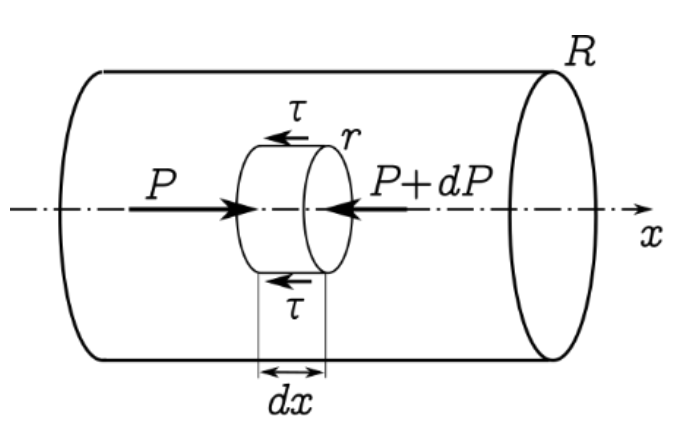
\includegraphics[width=0.43\textwidth]{Пуазейль.png}
        \caption{К выводу формулы Пуазейля}
    \end{wrapfigure}
    
    
    Выделим соосный трубе цилиндр некоторого радиуса $r$ и длины $d$. Поскольку при стационарном течении жидкость течёт без ускорения, сумма всех сил, действующих на жидкость в цилиндре, должна быть равна нулю.
    
    На жидкость внутри цилиндра действует направленная вдоль оси трубы сила давления:
    \begin{equation*}
    F_{1x} = -dP \cdot \pi r^2,
    \end{equation*}
    где $dP = P(x + d) - P(x) < 0$ — разность давлений в сечениях на торцах выделенного участка.
    \newpage
    На боковые поверхности цилиндра действует касательная сила вязкого трения:
    \begin{equation*}
    F_{2x} = -\tau \cdot 2\pi r d,
    \end{equation*}
    где согласно закону Ньютона:
    \begin{equation*}
    \tau = -\eta \frac{du}{dr}.
    \end{equation*}
    
    Из условия баланса сил $F_{1x} + F_{2x} = 0$ находим:
    \begin{equation*}
    \frac{dP}{dx} = \eta \cdot \frac{2}{r}  \frac{du}{dr}. 
    \end{equation*}
    
    В установившемся течении правая часть полученного выражения является функцией только радиуса $r$. В левой части находится градиент давления, который не зависит от $r$ вовсе, и, следовательно, обе части уравнения являются константами. Тогда, интегрируя, приходим к следующему.
    
    Во-первых, давление в трубе является линейно убывающей функцией координаты:
    \begin{equation*}
    P(x) = P_0 - \frac{\Delta P}{l} x. 
    \end{equation*}
    
    Во-вторых, профиль скорости является параболической функцией с максимумом на оси:
    \begin{equation*}
    u(r) = u_{\text{max}} - \frac{\Delta P}{4 l} r^2.
    \end{equation*}
    
    Для нахождения $v_{\text{max}}$ зададим граничное условие. Течения вязкой жидкости обычно используют так называемое условием прилипания: касательная скорость потока
    вблизи стенок считается равной скорости движения самих стенок. Физически
    это означает, что на молекулярном уровне стенки являются шероховатыми,
    так что при ударе о них молекулы в среднем полностью теряют направленную
    $x$-компоненту импульса. В рассматриваемой задаче стенки неподвижны, поэтому имеем
    \begin{equation*}
    v(r = R) = 0. 
    \end{equation*}
    
    Отсюда: $v_{\text{max}} = \frac{\Delta P}{4 L} R^2,$ и профиль скорости:

    \begin{equation*}
    u(r) = \frac{\Delta P}{4 l} (R^2 - r^2).
    \end{equation*}
    
    Интегрируя $v(r)$ по сечению трубы, найдём объёмный расход жидкости в зависимости от перепада давлений на концах:
    \begin{equation}
    Q = \int_0^R u(r) \cdot 2\pi r \, dr = \frac{\pi R^4 \Delta P}{8 \eta l}. 
    \end{equation}
    
    Это соотношение называют \textbf{формулой Пуазейля}. 
    Заметим, что средняя скорость потока при пуазейлевском течении, как видно из (1), оказывается
вдвое меньше максимальной:
    \begin{equation*}
    \bar{v} \equiv \frac{Q}{\pi R^2} = \frac{v_{\text{max}}}{2}.
    \end{equation*}
    
    Формула Пуазейля (1) позволяет определить вязкость газа по зависимости расхода от перепада давления в трубе и используется в качестве основной расчётной формулы в данной работе.

    \subsection{Вязкость газов}

        Рассмотрим механизм возникновения вязкости в газах.
    Молекулы газа участвуют как в направленном движении со средней скоростью потока $u$, так и в хаотическом тепловом движении, характеризующимся
    средней тепловой скоростью $\bar{v} = \sqrt{\frac{8k_{\text{Б}}T}{\pi m}}$ (здесь $m$ — масса молекулы). Молекулы могут свободно перемещаться между слоями и обмениваться друг с другом импульсами при столкновениях. Если в двух соседних слоях потоковыескорости различны, то такой обмен импульсом и приводит к эффективному возникновению силы трения между слоями. Исходя из приведенных соображений можно получить следующую
    оценку для коэффициента вязкости идеального газа:
    \begin{equation*}
    	\eta \sim \frac{1}{3}\rho \bar{v} \lambda,
    	\eqno(2)
    \end{equation*}
    где $\lambda$ — длина свободного пробега молекул газа относительно столкновений
    друг с другом. Как известно из молекулярно-кинетической теории, длина пробега определяется эффективным («газокинетическим») диаметром молекул $d$
    как $\lambda \sim 1/(n\pi d^2)$, где $n$ — объёмная концентрация газа. Видно, что $\lambda$ обратно пропорциональна плотности газа, поэтому, как следует из (2), вязкость газа не
    зависит от его плотности и определяется только температурой $T$. Данный
    вывод может показаться парадоксальным, поскольку в более плотном газе
    большее число молекул должно участвовать в передаче импульса между слоями, однако это компенсируется тем, что этот импульс передается на меньшее
    расстояние.
    \subsection{Турбулентность}
    Ламинарная картина течения наблюдается при относительно малых числах Рейнольдса, когда вязкие силы достаточны для того, чтобы погасить любые случайно возникшие возмущения потока. При превышении некоторого \textit{критического числа Рейнольдса} $Re > Re_{\text{кр}}$ течение Пуазейля становится \textit{неустойчивым}. В потоке начинают рождаться вихри, которые затем сносятся вниз по трубе (при докритических числах Рейнольдса такие вихри быстро затухают за счёт вязкости).
        \begin{wrapfigure}{r}{0.45\textwidth}
        \centering
        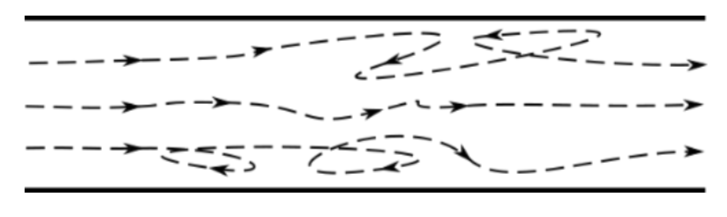
\includegraphics[width=0.43\textwidth]{turb.png}
        \caption{Пример траектории частиц жидкости при турбулентном течении}
    \end{wrapfigure}
    С дальнейшим увеличением $Re$
    количество вихрей возрастает и, взаимодействуя между собой, они порождают вихри всё меньшего размера, создавая таким образом сложную многомасштабную картин течения. Эта картина радикально отличается от ламинарной: в ней отсутствуют непрерывные
    линии тока, а слои жидкости постоянно \textit{перемешиваются}. Течение становится практически непредсказуемым, а скорость и давление испытывают значительные случайные \textit{флуктуации}.

    
    \subsubsection{Оценка турбулентного течения}
    
    В качестве примера воспользуемся аналогией с молекулярно-кинетической теорией и рассмотрим следующую упрощенную модель турбулентного
    течения. Примем, что флуктуации скорости в развитом турбулентном течении
    по порядку величины совпадают со средней скоростью потока $u \sim \bar{u}$. При
    этом элементы жидкости практически равномерно перемешиваются по сечению трубы, так что в качестве «длины пробега» жидкой частицы можно взять поперечный размер системы $R$. Тогда по аналогии с формулой (2) определим «турбулентную вязкость» как
    \begin{equation*}
    	\eta_{\text{турб}} \sim \rho \bar{u} R.
    	\eqno(3)
    \end{equation*}
    Далее по аналогии с выводом формулы Пуазейля запишем баланс сил в потоке, откуда получим оценку для средней скорости течения:
    \begin{equation*}
    	\eta_{\text{турб}}\frac{\bar{u}}{R} \cdot 2\pi rl \sim \pi R^2 \Delta P \ \  \xrightarrow{} \ \ \bar{u} \sim \frac{R^2 \Delta P}{\eta_{\text{турб}} l}
    \end{equation*}

    Подставляя сюда (3), находим скорость $\bar{u} \sim \sqrt{\frac{R \Delta P}{\rho l}}$
    и, как следствие, расход:
    \begin{equation*}
    	Q = \pi R^2 \bar{u} \sim R^{5/2}\sqrt{\frac{\Delta P}{\rho l}}.
    	\eqno(4)
    \end{equation*}
    Заметим, что эта теоретическая модель довольно груба и никак не учитывает сложную структуру турбулентного течения (например, не учитывается зависимость скорости потока $u$ от расстояния $r$ до оси трубы). 

    \section{Экспериментальная установка}
        Схема экспериментальной установки изображена на Рис. 3. Поток воздуха
    под давлением, немного превышающим атмосферное, поступает через газовый счётчик в тонкие металлические трубки. Воздух нагнетается компрессором, интенсивность его подачи регулируется краном К. Трубки снабжены
    съёмными заглушками на концах и рядом миллиметровых отверстий, к которым можно подключать микроманометр. В рабочем состоянии открыта заглушка на одной (рабочей) трубке, микроманометр подключён к двум её выводам, а все остальные отверстия плотно закрыты пробками.
    Перед входом в газовый счётчик установлен водяной U-образный манометр. Он служит для измерения давления газа на входе, а также предохраняет
    счётчик от выхода из строя. При превышении максимального избыточного
    давления на входе счётчика ($\sim$ 30 см вод. ст.) вода выплёскивается из трубки
    в защитный баллон Б, создавая шум и привлекая к себе внимание экспериментатора.
    \begin{figure}[h!]
            \centering
            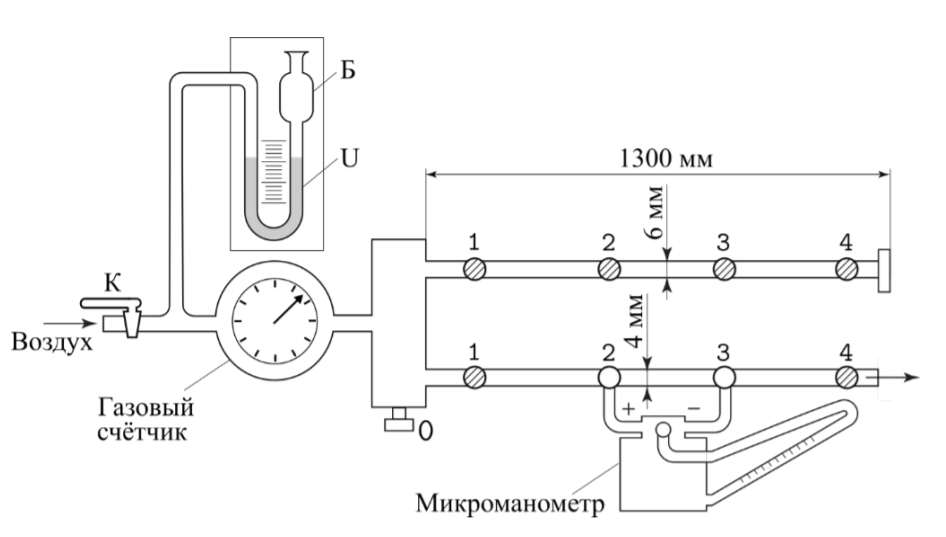
\includegraphics[scale=0.5]{expust.png}
            \caption{Экспериментальная установка}
     \end{figure} 
    
    \section{Приборы и данные}
    \begin{itemize}
        \item Термогигрометр с функцией отображения давления $testo \ 622$, погрешность измерения давления 3 гПа, температуры - 0,4 $^\circ C$, влажности - 2\% в диапазоне от 0 до 90 \%
        \item Микроманометр ММН-2400(5)-1б0, погрешность при различных K: 6 Па ($K = 0,2$), 9 Па ($K = 0,3$), 12 Па ($K = 0,4$), 18 Па ($K = 0,6$).
        \item Счетчик газовый барабанный модель ВИКС-1, погрешность измерения 1\%
    \end{itemize}

    \section{Ход работы}
    \begin{itemize}
        \item Начальные показания:
    $
    	t_\text{н} = 27,7 ^\circ C \ \ \ \  P_\text{н} = 996,9 \ \text{гПа} \ \ \ \  \varphi_\text{н} = 23,3 \%.
    $
        \item Показания в конце эксперимента:
    $
    	t_\text{к} = 27,3 ^\circ C \ \ \  P_\text{к} = 996,3 \ \text{гПа} \ \ \varphi_\text{к} = 21,2 \%,
    $
        \end{itemize}
    
    где $t$ - температруа в комнате, $P$ - давление, $\varphi$ - относительная влажность.\\

    \begin{enumerate}
        \item Ознакомились с устройством и характеристиками приборов (газового
    счетчика и спиртового микроманометра); провели их предварительную настройку и регулировку согласно техническому описанию установки.

        \item Провели предварительный запуск установки и убедились в ее работоспособности.

        \item Оценим критический расход и перепад давлений для каждой трубки. Для этого примем вязкость воздуха $\eta = 2 \cdot 10^{-5} \text{Па}\cdot c$, число Рейнольдса $Re_\text{кр} \approx 10^3$. Первая трубка диаметром $3,90 \pm 0,05$ мм:\\
        \begin{enumerate}
        
        \item Трубка 1 (d = 3.9 мм):
        \begin{itemize}
            \item $l = 0,50 \ \text{м}$: $\Delta P_\text{кр}^1 \approx 187 \ \text{Па}$
            \item $l = 0,90 \ \text{м}$: $\Delta P_\text{кр}^2 \approx 336 \ \text{Па}$
            \item $l = 1,20  \ \text{м}$: $\Delta P_\text{кр}^3 \approx 448 \ \text{Па}$
        \end{itemize}
    
        \item Трубка 2 (d = 5.25 мм):
        \begin{itemize}
            \item $l = 0,50 \  \text{м}$: $\Delta P_\text{кр}^4 \approx 76 \ \text{Па}$
            \item $l = 0,40 \ \text{м}$: $\Delta P_\text{кр}^5 \approx 61 \ \text{Па}$
            \item $l = 0,30 \ \text{м}$: $\Delta P_\text{кр}^6 \approx 46 \ \text{Па}$
        \end{itemize}
    
        \item Трубка 3 (d = 3.0 мм):
        \begin{itemize}
            \item $l = 0,20 \ \text{м}$: $\Delta P_\text{кр}^7 \approx 164 \ \text{Па}$
            \item $l = 0,40 \ \text{м}$: $\Delta P_\text{кр}^8 \approx 328 \ \text{Па}$
        \end{itemize}
    \end{enumerate}


        \item   Для трех трубок разных диаметров, меняя расположение микроманометра по длине трубки, будем менять расход сначала в пределах, когда течение еще ламинарное, а затем для турбулентного. Для каждого расхода будем фиксировать перепад давления. 
        Данные представлены в виде таблиц в приложении.


        \item   Для каждой серии построим график зависимости $Q(\Delta P)$ по методу $\chi^2$.

    Величина $\frac{\chi^2}{dof}$, где $dof$ (degrees of freedom) равно к $n-2$  характеризует степень согласия модели с данными. Если $\frac{\chi^2}{dof} \approx 1$, это означает хорошее согласие.\\
    \\
    Графики также представлены в приложении.


        \item По ламинарным участкам с помощью угловых коэфф. найдем вязкость воздуха $\eta$

\begin{equation*}
	\eta = \frac{\pi R^4}{8kl} = \frac{3,14 \cdot (\frac{3,9}{2})^4}{8\cdot 0,034 \cdot 0,5} \approx 2.004 \cdot 10^{-5} \, \text{Па} \cdot \text{с}
\end{equation*}
\begin{equation*}
	\sigma_\eta = \eta \sqrt{(\frac{4\sigma_R}{R})^2 + (\frac{\sigma_k}{k})^2} = 2.004 \cdot 10^{-5} \sqrt{(0,05)^2 + (0,008)^2} \approx 0,104 \cdot 10^{-5} \, \text{Па} \cdot \text{с}
\end{equation*}

            \begin{table}[h!]
        \centering
        
        \begin{tabular}{|c|c|c|c|}
        \hline
        № & $\eta, \cdot 10^{-5}~\text{Па} \cdot \text{с}$ & $\sigma_\eta, \cdot 10^{-5}~\text{Па} \cdot \text{с}$ & $\varepsilon_\eta, \%$ \\
        \hline
        1 & 2.004 & 0.104 & 5.20 \\ \hline
        2 & 1.951 & 0.101 & 5.15 \\ \hline
        3 & 1.931 & 0.099 & 5.17 \\ \hline
        4 & 2.019 & 0.080 & 3.96 \\ \hline
        5 & 2.194 & 0.087 & 3.94 \\ \hline
        6 & 2.099 & 0.082 & 3.89 \\ \hline
        7 & 0.738 & 0.104 & 14.06 \\ \hline
        8 & 0.779 & 0.111 & 14.23 \\ \hline
        \end{tabular}
        \caption{Результаты расчёта коэффициента динамической вязкости}
        \end{table}

    \item Для того чтобы рассчитать число Рейнольдса, найдём точки пересечения графиков для соответствубщих трубок и соответсвующих диаметров. Построим линейное приближение для турбулентного течения, графики также представлены в приложении.
    По границам перехода от ламинарного участка к турбулентному рассчитаем число Рейнольдса $Re_\text{кр}$:
\begin{equation*}
	Re_\text{кр} = \frac{P \mu_{\text{воз}} Q_\text{кр}}{R_\text{газ}T \eta \pi R}
\end{equation*}

\begin{table}[h!]
    \centering
    \begin{tabular}{|c|c|}
        \hline
        \textnumero & $Re_\text{кр}$ \\ \hline
        1 & 898 \\ \hline
        2 & 969 \\ \hline
        3 & 929 \\ \hline
        4 & 891 \\ \hline
        5 & 803 \\ \hline
        6 & 910 \\ \hline
        7 & 2627 \\ \hline
        8 & 2189 \\ \hline
    \end{tabular}
    \captionof{table}{Критические значения числа Рейнольдса для серий 1--8.}
\end{table}
        
    \end{enumerate}

    \section{Результаты и обсуждения}
\begin{enumerate}
\item По графикам 1-3 видно, что расход прямо пропорционален перепаду давления, точки хорошо ложатся на прямую при ламинарном течении. Сравним полученные экспериментально коэффициенты вязкости с табличным значением $\eta_{\text{табл}} 1,832 \cdot 10^{-5} \, \text{Па}. \cdot \text{с}$
\begin{table}[h!]
    \centering
    \begin{tabular}{|c|c|c|c|c|}
        \hline
        $\eta, \cdot 10^{-5} \, \text{Па} \cdot \text{с}$ & $\sigma_{\eta_{\text{эксп}}}, \cdot 10^{-5} \, \text{Па} \cdot \text{с}$ & $\sigma_{\eta_{\text{табл}}}, \cdot 10^{-5} \, \text{Па} \cdot \text{с}$ & $\varepsilon_{\eta_{\text{эксп}}}, \%$ & $\varepsilon_{\eta_{\text{табл}}}, \%$ \\
        \hline
        2.004 & 0.104  & 0,175 & 5.20  & 9,53 \\ \hline
        1.951 & 0.101  & 0,119 & 5.15  & 6,48 \\ \hline
        1.931 & 0.099  & 0,094 & 5.17  & 5,11 \\ \hline
        2.019 & 0.080  & 0,152 & 3.96  & 8,28 \\ \hline
        2.194 & 0.087  & 0,381 & 3.94  & 20,78 \\ \hline
        2.099 & 0.082  & 0,307 & 3.89  & 16,76 \\ \hline
        0.738 & 0.104  & 1,025 & 14.06 & 55,95 \\ \hline
        0.779 & 0.111  & 1,055 & 14.23 & 57,60 \\ \hline
    \end{tabular}
    \captionof{table}{Таблица 19. Сравнение экспериментальных и табличных погрешностей вязкости}
\end{table}
По таблице видно, что коэффициенты, полученные в сериях с трьетей трубкой отличаются более чем в 2 раза. Можем предположить, что это связано с тем, что длина трубки была меньше, чем рассчитанная длина установления давления, поэтому на этом участке течение не подчиняется закону Пуазейля. Также перепад давления на этой трубке довольно мал, что приводит к большой относительной погрешности. Остальные коэффициенты совпадают с табличными с хорошей точностью. Это подтверждает тот факт, что значение вязкости не зависит от диаметра трубки.
\item По графикам 4-9 можем убедиться, что при турбулентном течении расход действительно зависит от корня перепада давления.
\item Поскольку определить точно границу перехода от ламинарного течения к турбулентному в данном опыте довольно трудно, мы воспользовались приближением и нашли эти точки как точки пересечения графиков. 

\end{enumerate}
\section{Выводы}

 Провели измерения перепада давления от расхода газа для трех трубок разного диаметра и разной длины. Построили графики зависимости $Q(\Delta P)$, с помощью них нашли коэффициенты вязкости воздуха для наших параметров окружающей среды. Убедились в том, что вязкость не зависит от диаметра трубки. Оценили критические значения числа Рейнольдса. 

% \newpage
    \section{Приложение}

\begin{table}[h!]
\centering
\begin{minipage}{0.48\textwidth}
\centering
    \begin{tabular}{|c|c|c|c|c|}
        \hline
        $Q$, $\frac{\text{л}}{\text{мин}}$ & $\sigma_Q$, $\frac{\text{л}}{\text{мин}}$  & $\Delta P$, Па & $\sigma_{\Delta P}$, Па & $\varepsilon_{\Delta P}$, \% \\
        \hline
        1.352 & 0.014 & 37 & 6 & 16.2 \\ \hline
        2.363 & 0.024 & 64 & 6 & 9.3 \\ \hline
        2.894 & 0.029 & 78 & 6 & 7.7 \\ \hline
        3.897 & 0.039 & 107 & 6 & 5.6 \\ \hline
        4.468 & 0.045 & 134 & 6 & 4.5 \\ \hline
        4.945 & 0.049 & 140 & 6 & 4.3 \\ \hline
        5.483 & 0.055 & 162 & 6 & 3.7 \\ \hline
    \end{tabular}
    \caption{$d=3,90 \pm 0,05$ мм; $l = 0,5$ м; $K = 0,2$}
\end{minipage}
\hfill
\begin{minipage}{0.48\textwidth}
\centering
    \begin{tabular}{|c|c|c|c|c|}
        \hline
        $Q$, $\frac{\text{л}}{\text{мин}}$ & $\sigma_Q$, $\frac{\text{л}}{\text{мин}}$  & $\Delta P$, Па & $\sigma_{\Delta P}$, Па & $\varepsilon_{\Delta P}$, \% \\
        \hline
        1.28 & 0.013 & 58 & 9 & 15.4 \\ \hline
        2.788 & 0.028 & 120 & 9 & 7.5 \\ \hline
        3.226 & 0.032 & 158 & 9 & 5.7 \\ \hline
        3.581 & 0.036 & 175 & 9 & 5.1 \\ \hline
        4.138 & 0.041 & 201 & 9 & 4.5 \\ \hline
        4.58 & 0.046 & 210 & 9 & 4.3 \\ \hline
        5.04 & 0.050 & 257 & 9 & 3.5 \\ \hline
        5.452 & 0.055 & 292 & 9 & 3.1 \\ \hline
    \end{tabular}
    \caption{$d = 3,90 \pm 0,05$ мм; $l = 0,9$ м; $K = 0,3$}
\end{minipage}
\end{table}

\begin{table}[h!]
\centering
\begin{minipage}{0.48\textwidth}
\centering
    \begin{tabular}{|c|c|c|c|c|}
        \hline
        $Q$, $\frac{\text{л}}{\text{мин}}$ & $\sigma_Q$, $\frac{\text{л}}{\text{мин}}$  & $\Delta P$, Па & $\sigma_{\Delta P}$, Па & $\varepsilon_{\Delta P}$, \% \\
        \hline
        1.024 & 0.010 & 62 & 12 & 19.2 \\ \hline
        2.236 & 0.022 & 140 & 12 & 8.6 \\ \hline
        2.584 & 0.026 & 168 & 12 & 7.2 \\ \hline
        3.212 & 0.032 & 206 & 12 & 5.8 \\ \hline
        3.621 & 0.036 & 234 & 12 & 5.1 \\ \hline
        4.404 & 0.044 & 292 & 12 & 4.1 \\ \hline
        5.166 & 0.052 & 355 & 12 & 3.4 \\ \hline
    \end{tabular}
    \caption{$d = 3,90 \pm 0,05$ мм; $l = 1,2$ м; $K = 0,4$}
\end{minipage}
\hfill
\begin{minipage}{0.48\textwidth}
\centering
    \begin{tabular}{|c|c|c|c|c|}
        \hline
        $Q$, $\frac{\text{л}}{\text{мин}}$ & $\sigma_Q$, $\frac{\text{л}}{\text{мин}}$  & $\Delta P$, Па & $\sigma_{\Delta P}$, Па & $\varepsilon_{\Delta P}$, \% \\
        \hline
        7.083 & 0.071 & 308 & 6 & 1.9 \\ \hline
        7.943 & 0.079 & 385 & 9 & 2.3 \\ \hline
        8.533 & 0.085 & 447 & 9 & 2.0 \\ \hline
        9.395 & 0.094 & 540 & 9 & 1.7 \\ \hline
        9.814 & 0.098 & 587 & 9 & 1.5 \\ \hline
        10.052 & 0.101 & 610 & 9 & 1.5 \\ \hline
        10.755 & 0.108 & 701 & 9 & 1.3 \\ \hline
    \end{tabular}
    \caption{$d = 3,90 \pm 0,05$ мм; $l = 0,5$ м; $K = 0,3$}
\end{minipage}
\end{table}

\begin{table}[h!]
\centering
\begin{minipage}{0.48\textwidth}
\centering
    \begin{tabular}{|c|c|c|c|c|}
        \hline
        $Q$, $\frac{\text{л}}{\text{мин}}$ & $\sigma_Q$, $\frac{\text{л}}{\text{мин}}$  & $\Delta P$, Па & $\sigma_{\Delta P}$, Па & $\varepsilon_{\Delta P}$, \% \\
        \hline
        7.058 & 0.071 & 510 & 12 & 2.4 \\ \hline
        7.799 & 0.078 & 686 & 12 & 1.7 \\ \hline
        8.452 & 0.085 & 791 & 12 & 1.5 \\ \hline
        8.793 & 0.088 & 857 & 12 & 1.4 \\ \hline
        9.087 & 0.091 & 927 & 12 & 1.3 \\ \hline
        9.319 & 0.093 & 978 & 12 & 1.2 \\ \hline
        9.814 & 0.098 & 1064 & 12 & 1.1 \\ \hline
    \end{tabular}
    \caption{$d = 3,90 \pm 0,05$ мм; $l = 0,9$ м; $K = 0,4$}
\end{minipage}
\hfill
\begin{minipage}{0.48\textwidth}
\centering
    \begin{tabular}{|c|c|c|c|c|}
        \hline
        $Q$, $\frac{\text{л}}{\text{мин}}$ & $\sigma_Q$, $\frac{\text{л}}{\text{мин}}$  & $\Delta P$, Па & $\sigma_{\Delta P}$, Па & $\varepsilon_{\Delta P}$, \% \\
        \hline
        7.632 & 0.076 & 839 & 18 & 2.1 \\ \hline
        8.113 & 0.081 & 950 & 18 & 1.9 \\ \hline
        8.441 & 0.084 & 1020 & 18 & 1.8 \\ \hline
        8.895 & 0.089 & 1125 & 18 & 1.6 \\ \hline
        9.575 & 0.096 & 1288 & 18 & 1.4 \\ \hline
        9.313 & 0.093 & 1235 & 18 & 1.5 \\ \hline
        9.868 & 0.099 & 1398 & 18 & 1.3 \\ \hline
    \end{tabular}
    \caption{$d = 3,90 \pm 0,05$ мм; $l = 1,2$ м; $K = 0,6$}
\end{minipage}
\end{table}

\begin{table}[h!]
\centering
\begin{minipage}{0.48\textwidth}
\centering
    \begin{tabular}{|c|c|c|c|c|}
        \hline
        $Q$, $\frac{\text{л}}{\text{мин}}$ & $\sigma_Q$, $\frac{\text{л}}{\text{мин}}$  & $\Delta P$, Па & $\sigma_{\Delta P}$, Па & $\varepsilon_{\Delta P}$, \% \\
        \hline
        2.58 & 0.026 & 19 & 6 & 30.8 \\ \hline
        3.31 & 0.033 & 27 & 6 & 22.0 \\ \hline
        5.399 & 0.054 & 45 & 6 & 13.4 \\ \hline
        6.638 & 0.066 & 55 & 6 & 11.0 \\ \hline
        4.485 & 0.045 & 37 & 6 & 16.2 \\ \hline
        6.91 & 0.069 & 58 & 6 & 10.3 \\ \hline
        5.116 & 0.051 & 43 & 6 & 14.0 \\ \hline
    \end{tabular}
    \caption{$d = 5,25 \pm 0,05$ мм; $l = 0,5$ м; $K = 0,2$}
\end{minipage}
\hfill
\begin{minipage}{0.48\textwidth}
\centering
    \begin{tabular}{|c|c|c|c|c|}
        \hline
        $Q$, $\frac{\text{л}}{\text{мин}}$ & $\sigma_Q$, $\frac{\text{л}}{\text{мин}}$  & $\Delta P$, Па & $\sigma_{\Delta P}$, Па & $\varepsilon_{\Delta P}$, \% \\
        \hline
        2.478 & 0.025 & 16 & 6 & 38.5 \\ \hline
        3.383 & 0.034 & 23 & 6 & 25.7 \\ \hline
        5.441 & 0.054 & 39 & 6 & 15.4 \\ \hline
        4.226 & 0.042 & 29 & 6 & 20.5 \\ \hline
        6.386 & 0.064 & 47 & 6 & 12.8 \\ \hline
        6.964 & 0.070 & 51 & 6 & 11.8 \\ \hline
        7.815 & 0.078 & 58 & 6 & 10.3 \\ \hline
    \end{tabular}
    \caption{$d = 5,25 \pm 0,05$ мм; $l = 0,4$ м; $K = 0,2$}
\end{minipage}
\end{table}

\begin{table}[h!]
\centering
\begin{minipage}{0.48\textwidth}
\centering
    \begin{tabular}{|c|c|c|c|c|}
        \hline
        $Q$, $\frac{\text{л}}{\text{мин}}$ & $\sigma_Q$, $\frac{\text{л}}{\text{мин}}$  & $\Delta P$, Па & $\sigma_{\Delta P}$, Па & $\varepsilon_{\Delta P}$, \% \\
        \hline
        1.535 & 0.015 & 8 & 6 & 77.0 \\ \hline
        2.738 & 0.027 & 14 & 6 & 44.0 \\ \hline
        3.759 & 0.038 & 19 & 6 & 30.8 \\ \hline
        4.331 & 0.043 & 23 & 6 & 25.7 \\ \hline
        4.922 & 0.049 & 27 & 6 & 22.0 \\ \hline
        6.245 & 0.062 & 35 & 6 & 17.1 \\ \hline
        6.811 & 0.068 & 39 & 6 & 15.4 \\ \hline
    \end{tabular}
    \caption{$d=5,25 \pm 0,05$ мм; $l = 0,3$ м; $K = 0,2$}
\end{minipage}
\hfill
\begin{minipage}{0.48\textwidth}
\centering
    \begin{tabular}{|c|c|c|c|c|}
        \hline
        $Q$, $\frac{\text{л}}{\text{мин}}$ & $\sigma_Q$, $\frac{\text{л}}{\text{мин}}$  & $\Delta P$, Па & $\sigma_{\Delta P}$, Па & $\varepsilon_{\Delta P}$, \% \\
        \hline
        9.067 & 0.091 & 109 & 6 & 5.5 \\ \hline
        9.735 & 0.097 & 134 & 6 & 4.5 \\ \hline
        10.334 & 0.103 & 156 & 6 & 3.8 \\ \hline
        11.379 & 0.114 & 185 & 6 & 3.2 \\ \hline
        12.416 & 0.124 & 218 & 6 & 2.7 \\ \hline
        13.158 & 0.132 & 249 & 6 & 2.4 \\ \hline
        13.935 & 0.139 & 267 & 6 & 2.2 \\ \hline
    \end{tabular}
    \caption{$d = 5,25 \pm 0,05$ мм; $l = 0,5$ м; $K = 0,2$}
\end{minipage}
\end{table}

\begin{table}[h!]
\centering
\begin{minipage}{0.48\textwidth}
\centering
    \begin{tabular}{|c|c|c|c|c|}
        \hline
        $Q$, $\frac{\text{л}}{\text{мин}}$ & $\sigma_Q$, $\frac{\text{л}}{\text{мин}}$  & $\Delta P$, Па & $\sigma_{\Delta P}$, Па & $\varepsilon_{\Delta P}$, \% \\
        \hline
        9.305 & 0.093 & 103 & 6 & 5.8 \\ \hline
        10.103 & 0.101 & 127 & 6 & 4.7 \\ \hline
        11.228 & 0.112 & 154 & 6 & 3.9 \\ \hline
        11.921 & 0.119 & 173 & 6 & 3.5 \\ \hline
        12.679 & 0.127 & 193 & 6 & 3.1 \\ \hline
        13.052 & 0.131 & 205 & 6 & 2.9 \\ \hline
        13.583 & 0.136 & 222 & 6 & 2.7 \\ \hline
    \end{tabular}
    \caption{$d=5,25 \pm 0,05$ мм; $l = 0,4$ м; $K = 0,2$}
\end{minipage}
\hfill
\begin{minipage}{0.48\textwidth}
\centering
    \begin{tabular}{|c|c|c|c|c|}
        \hline
        $Q$, $\frac{\text{л}}{\text{мин}}$ & $\sigma_Q$, $\frac{\text{л}}{\text{мин}}$  & $\Delta P$, Па & $\sigma_{\Delta P}$, Па & $\varepsilon_{\Delta P}$, \% \\
        \hline
        10.947 & 0.109 & 92 & 6 & 6.6 \\ \hline
        11.684 & 0.117 & 103 & 6 & 5.8 \\ \hline
        12.177 & 0.122 & 113 & 6 & 5.3 \\ \hline
        12.662 & 0.127 & 119 & 6 & 5.0 \\ \hline
        13.137 & 0.131 & 129 & 6 & 4.7 \\ \hline
        13.591 & 0.136 & 136 & 6 & 4.4 \\ \hline
        14.102 & 0.141 & 144 & 6 & 4.2 \\ \hline
    \end{tabular}
    \caption{$d=5,25 \pm 0,05$ мм; $l = 0,3$ м; $K = 0,2$}
\end{minipage}
\end{table}

\begin{table}[h!]
\centering
\begin{minipage}{0.48\textwidth}
\centering
    \begin{tabular}{|c|c|c|c|c|}
        \hline
        $Q$, $\frac{\text{л}}{\text{мин}}$ & $\sigma_Q$, $\frac{\text{л}}{\text{мин}}$  & $\Delta P$, Па & $\sigma_{\Delta P}$, Па & $\varepsilon_{\Delta P}$, \% \\
        \hline
        1.118 & 0.011 & 10 & 6 & 61.6 \\ \hline
        1.901 & 0.019 & 19 & 6 & 30.8 \\ \hline
        1.26 & 0.013 & 12 & 6 & 51.3 \\ \hline
        1.54 & 0.015 & 14 & 6 & 44.0 \\ \hline
        2.347 & 0.023 & 23 & 6 & 25.7 \\ \hline
        2.733 & 0.027 & 29 & 6 & 20.5 \\ \hline
        3.197 & 0.032 & 37 & 6 & 16.2 \\ \hline
    \end{tabular}
    \caption{$d = 3,0 \pm 0,1$ мм; $l = 0,2$ м; $K = 0,2$}
\end{minipage}
\hfill
\begin{minipage}{0.48\textwidth}
\centering
    \begin{tabular}{|c|c|c|c|c|}
        \hline
       $Q$, $\frac{\text{л}}{\text{мин}}$ & $\sigma_Q$, $\frac{\text{л}}{\text{мин}}$  & $\Delta P$, Па & $\sigma_{\Delta P}$, Па & $\varepsilon_{\Delta P}$, \% \\
        \hline
        0.561 & 0.006 & 12 & 6 & 51.3 \\ \hline
        1.107 & 0.011 & 25 & 6 & 23.7 \\ \hline
        1.574 & 0.016 & 39 & 6 & 15.4 \\ \hline
        1.86 & 0.019 & 47 & 6 & 12.8 \\ \hline
        2.135 & 0.021 & 51 & 6 & 11.8 \\ \hline
    \end{tabular}
    \caption{$d = 3,0 \pm 0,1$ мм; $l = 0,4$ м; $K = 0,2$}
\end{minipage}
\end{table}

\begin{table}[h!]
\centering
\begin{minipage}{0.48\textwidth}
\centering
    \begin{tabular}{|c|c|c|c|c|}
        \hline
        $Q$, $\frac{\text{л}}{\text{мин}}$ & $\sigma_Q$, $\frac{\text{л}}{\text{мин}}$  & $\Delta P$, Па & $\sigma_{\Delta P}$, Па & $\varepsilon_{\Delta P}$, \% \\
        \hline
        6.038 & 0.060 & 97 & 6 & 6.2 \\ \hline
        6.803 & 0.068 & 113 & 6 & 5.3 \\ \hline
        7.139 & 0.071 & 125 & 6 & 4.8 \\ \hline
        8.375 & 0.084 & 156 & 6 & 3.8 \\ \hline
        8.966 & 0.090 & 175 & 6 & 3.4 \\ \hline
        9.56 &  0.096  & 203 & 6 & 3.0 \\ \hline
        10.179 &0.102 & 222 & 6 & 2.7 \\ \hline
    \end{tabular}
    \caption{$d = 3,0 \pm 0,1$ мм; $l = 0,2$ м; $K = 0,2$}
\end{minipage}
\hfill
\begin{minipage}{0.48\textwidth}
\centering
    \begin{tabular}{|c|c|c|c|c|}
        \hline
        $Q$, $\frac{\text{л}}{\text{мин}}$ & $\sigma_Q$, $\frac{\text{л}}{\text{мин}}$ & $\Delta P$, Па & $\sigma_{\Delta P}$, Па & $\varepsilon_{\Delta P}$, \% \\
        \hline
        5.202 & 0.052 & 187 & 6 & 3.2 \\ \hline
        5.836 & 0.058 & 228 & 6 & 2.6 \\ \hline
        6.194 & 0.062 & 245 & 6 & 2.4 \\ \hline
        6.951 & 0.070 & 310 & 6 & 1.9 \\ \hline
        7.662 & 0.077 & 364 & 6 & 1.6 \\ \hline
    \end{tabular}
    \caption{$d = 3,0 \pm 0,1$ мм; $l = 0,4$ м; $K = 0,2$}
\end{minipage}
\end{table}

% \newpage

% \subsection{Графики}

    \begin{figure}[h!]
    \centering{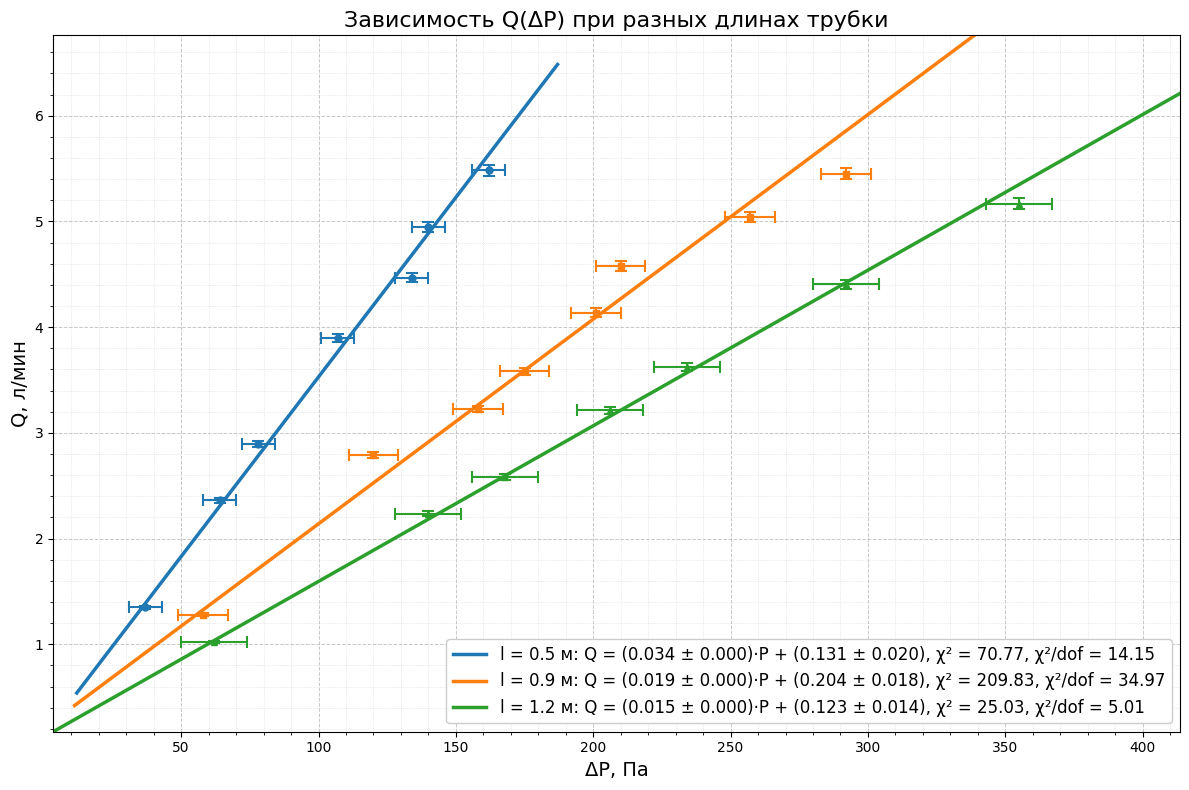
\includegraphics[width=0.95\textwidth]{graphs/lam1.png}}
    \caption[]{ Ламинарное течение, первая трубка d = 3.9 \text{мм}}
    \end{figure}

    \begin{figure}[h!]
    \centering{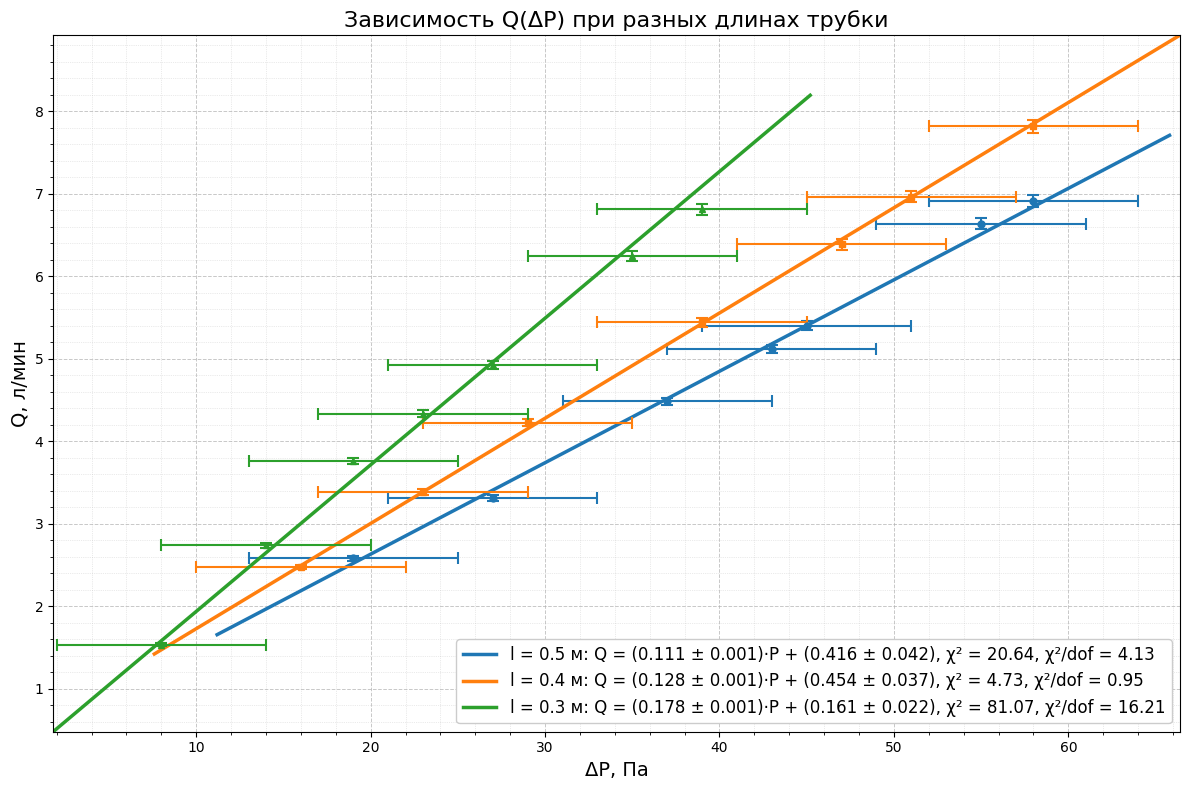
\includegraphics[width=0.95\textwidth]{graphs/lam2.png}}
    \caption[]{ Ламинарное течение, вторая трубка d = 5.25 \text{мм}}
    \end{figure}

    \begin{figure}[h!]
    \centering{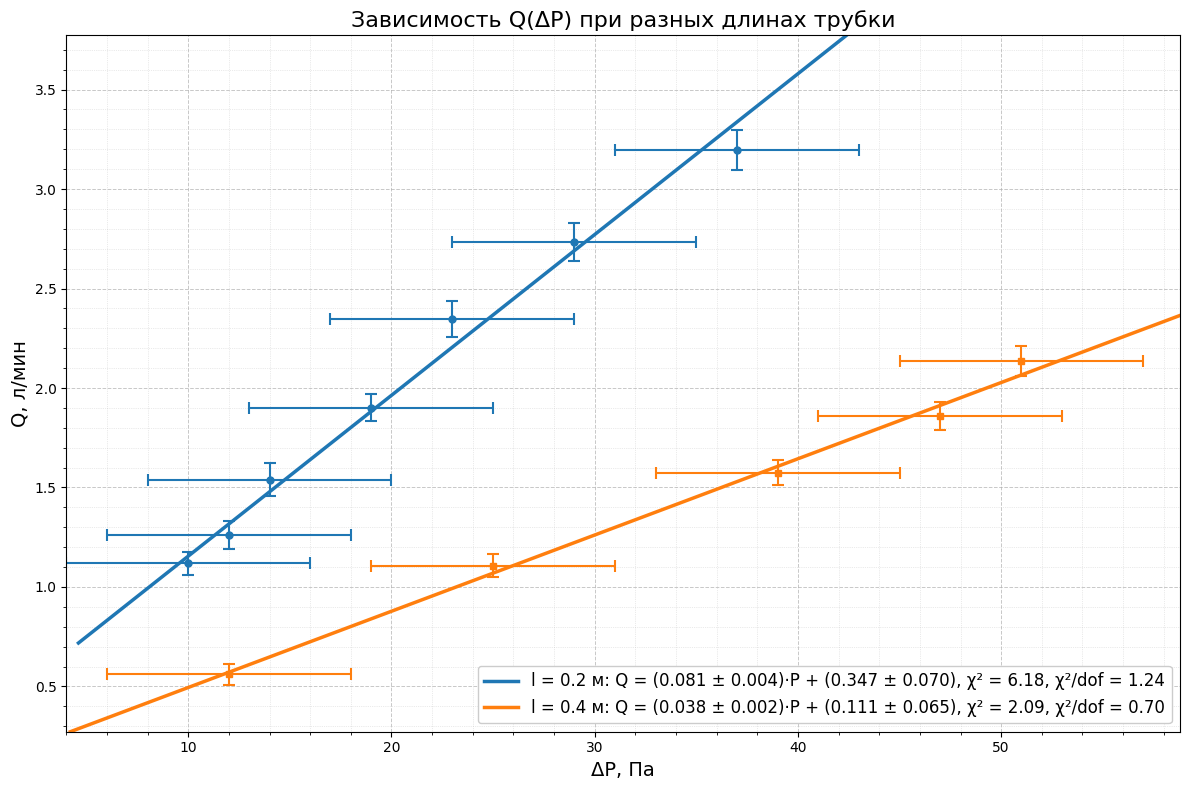
\includegraphics[width=0.95\textwidth]{graphs/lam3.png}}
    \caption[]{ Ламинарное течение, третья трубка d = 3.0 \text{мм}}
    \end{figure}

    \begin{figure}[h!]
    \centering{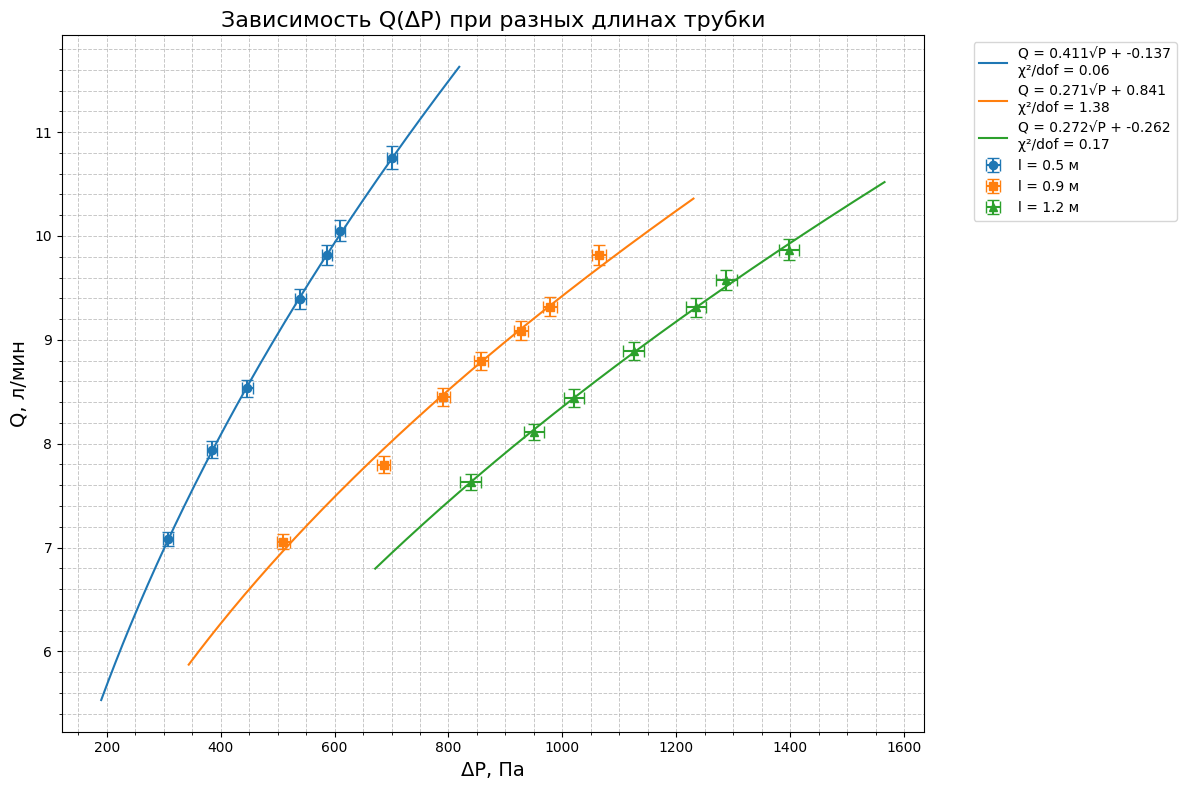
\includegraphics[width=0.95\textwidth]{graphs/sqrt-turb1.png}}
    \caption[]{ Турбулентное течение, первая трубка d = 3.9 \text{мм}}
    \end{figure}

    \begin{figure}[h!]
    \centering{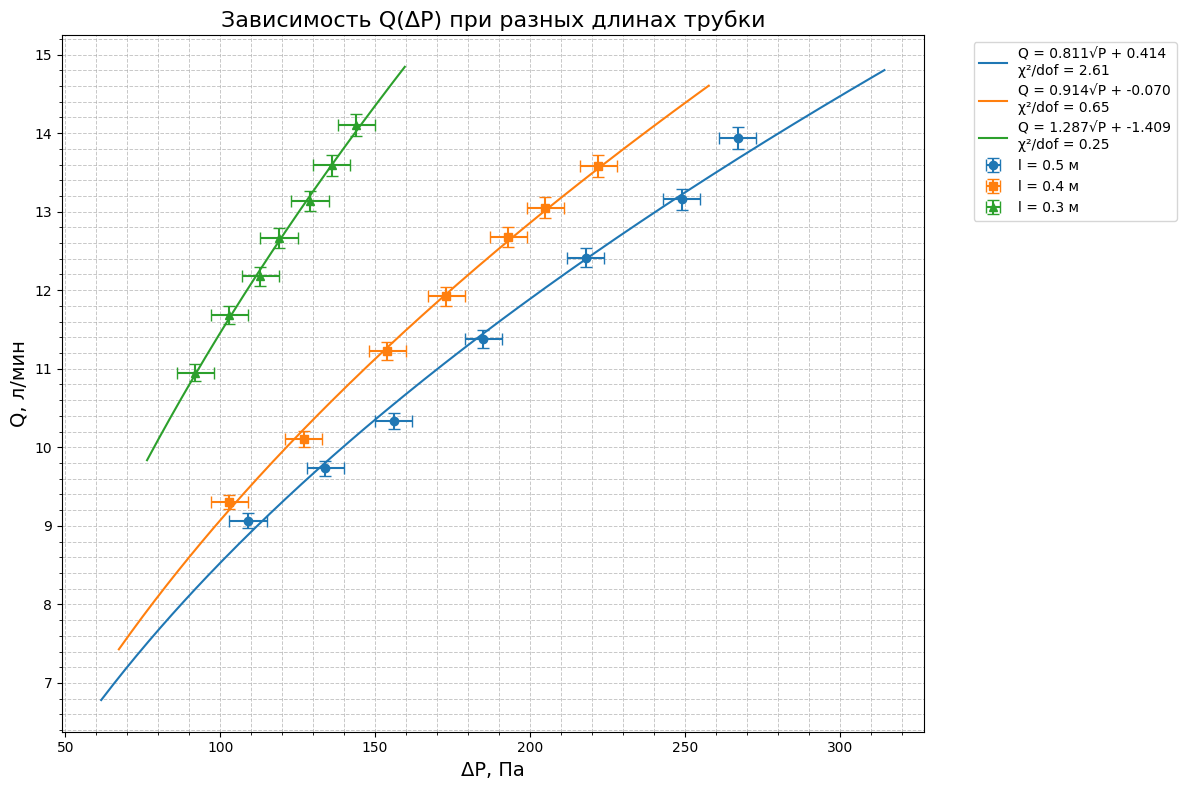
\includegraphics[width=0.95\textwidth]{graphs/sqrt-turb2.png}}
    \caption[]{ Турбулентное течение, вторая трубка d = 5.25 \text{мм}}
    \end{figure}

    \begin{figure}[h!]
    \centering{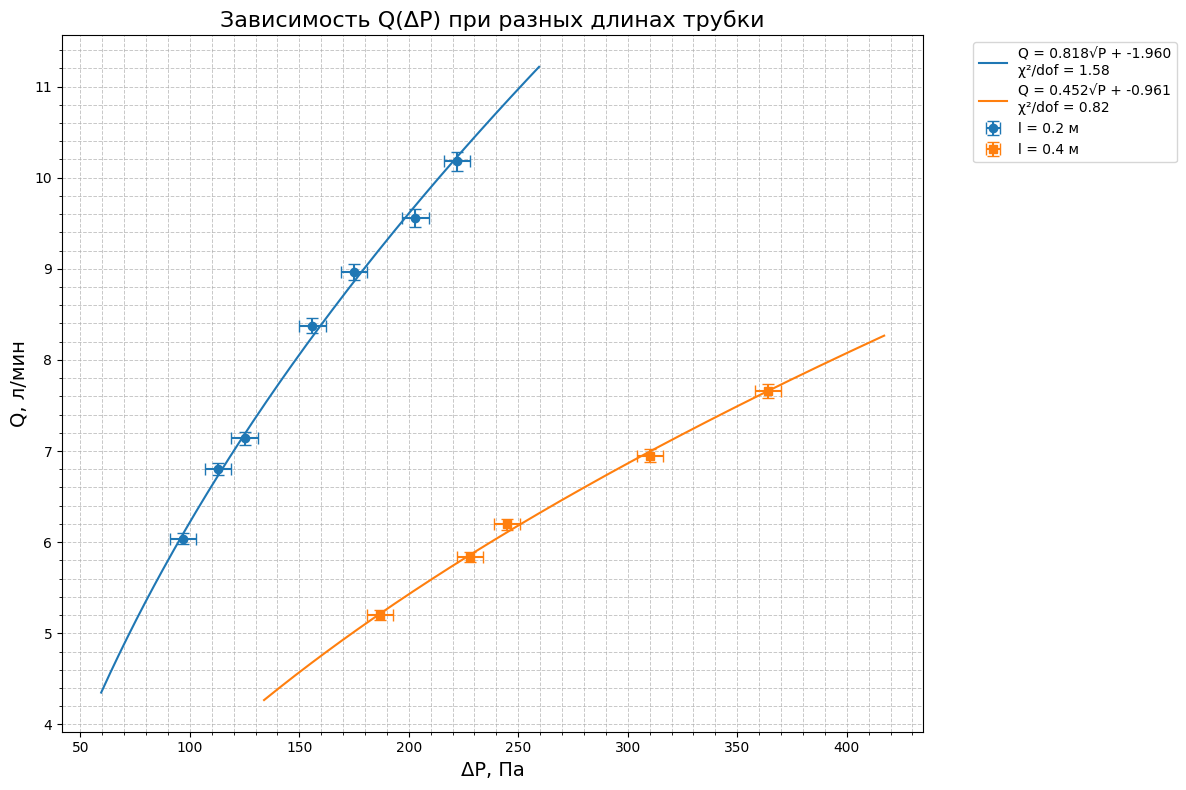
\includegraphics[width=0.95\textwidth]{graphs/sqrt-turb3.png}}
    \caption[]{ Турбулентное течение, третья трубка d = 3.0 \text{мм}}
    \end{figure}

    \begin{figure}[h!]
    \centering{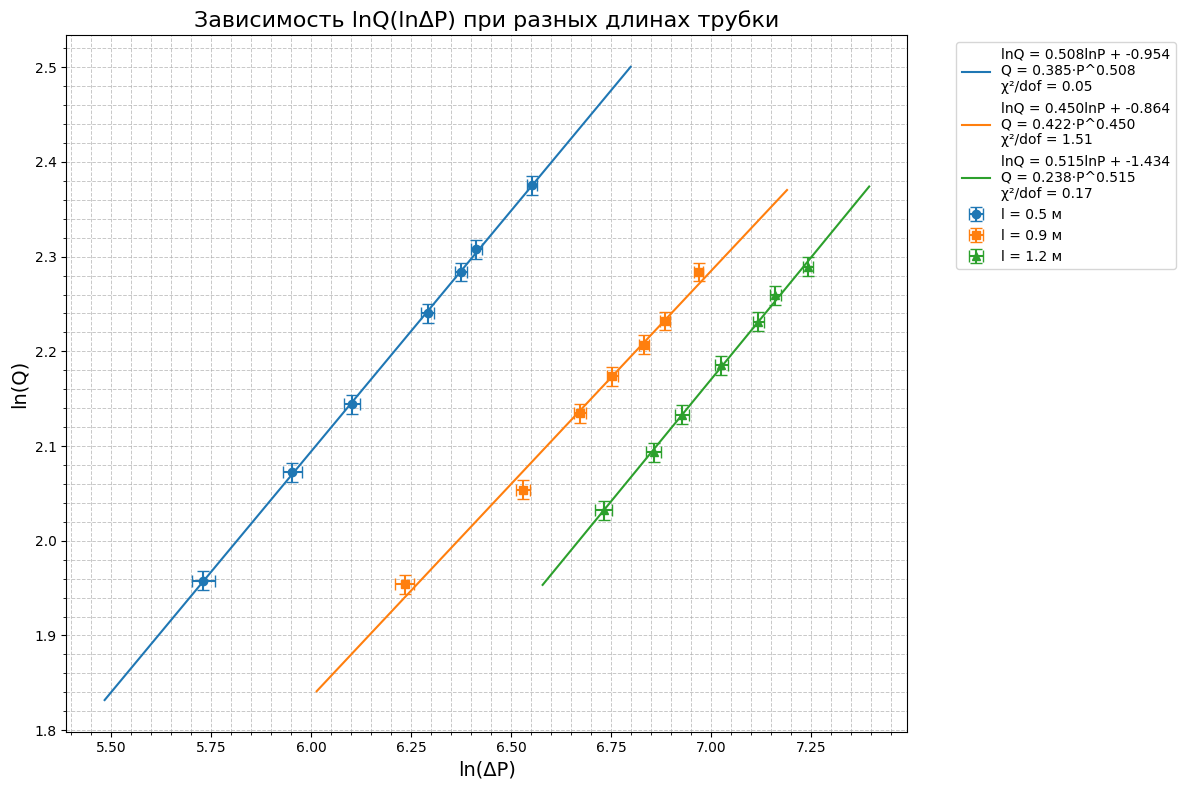
\includegraphics[width=0.95\textwidth]{graphs/ln-turb1.png}}
    \caption[]{ Турбулентное течение, первая трубка d = 3.9 \text{мм}}
    \end{figure}

    \begin{figure}[h!]
    \centering{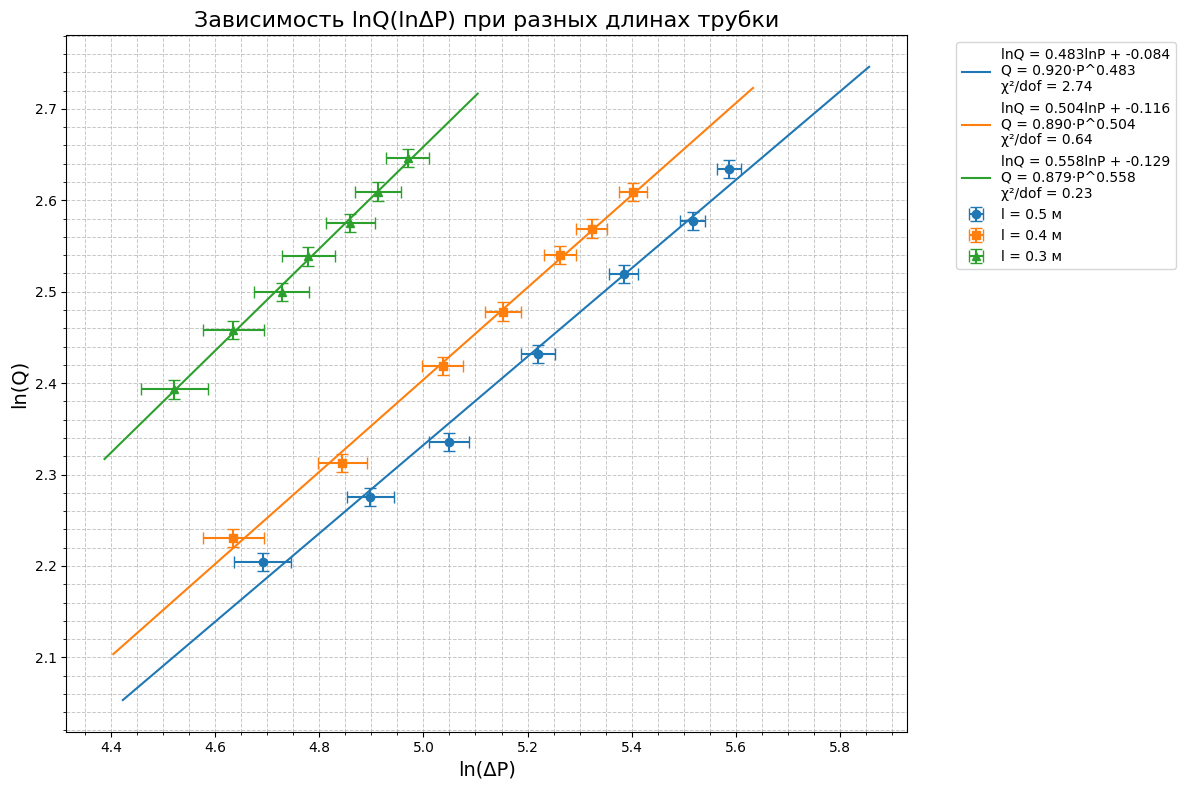
\includegraphics[width=0.95\textwidth]{graphs/ln-turb2.png}}
    \caption[]{ Турбулентное течение, вторая трубка d = 5.25 \text{мм}}
    \end{figure}

    \begin{figure}[h!]
    \centering{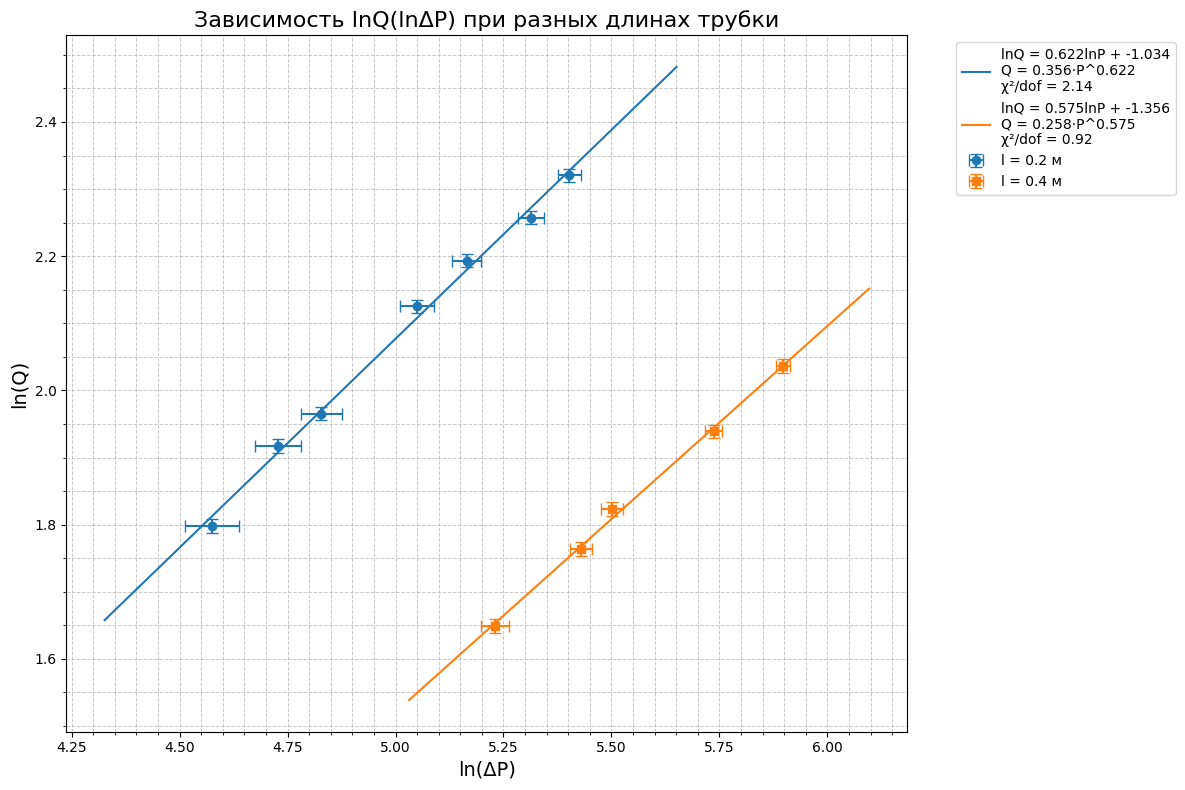
\includegraphics[width=0.95\textwidth]{graphs/ln-turb3.png}}
    \caption[]{ Турбулентное течение, третья трубка d = 3.0 \text{мм}}
    \end{figure}

    \begin{figure}[h!]
    \centering{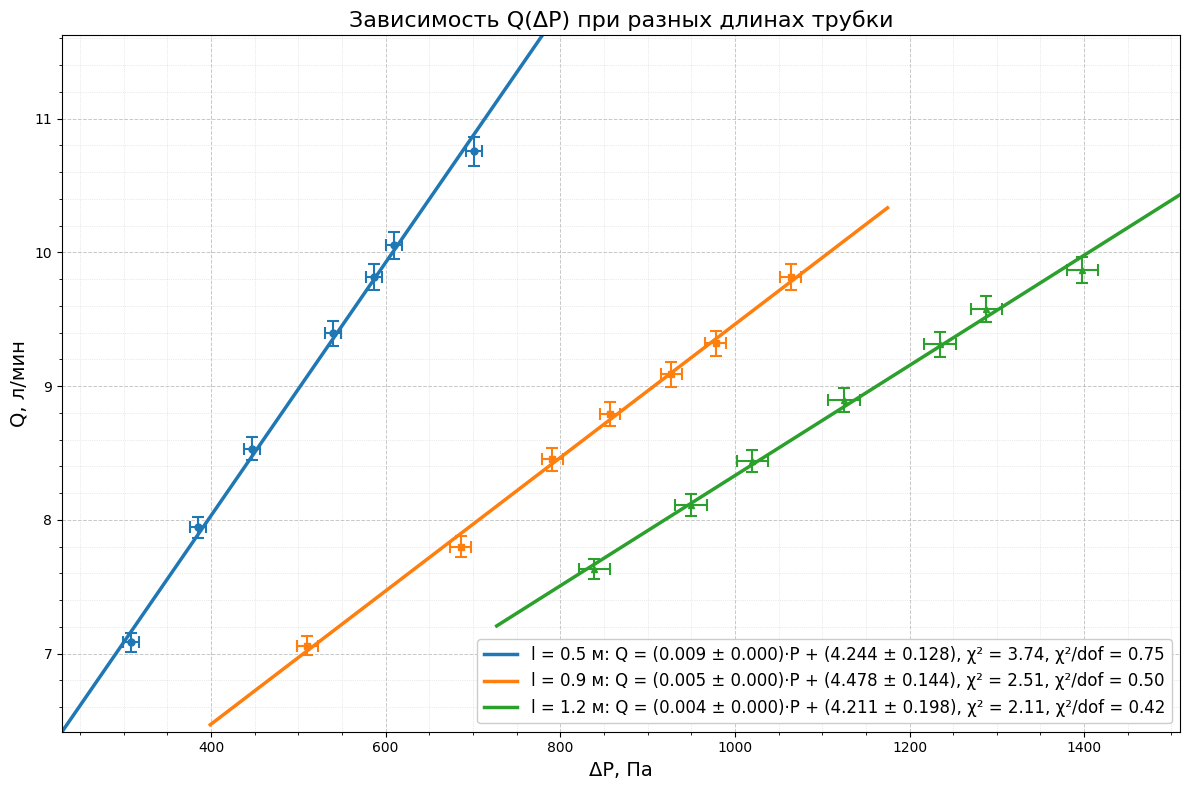
\includegraphics[width=0.95\textwidth]{graphs/turb1.png}}
    \caption[]{ Турбулентное течение, первая трубка d = 3.9 \text{мм}}
    \end{figure}

    \begin{figure}[h!]
    \centering{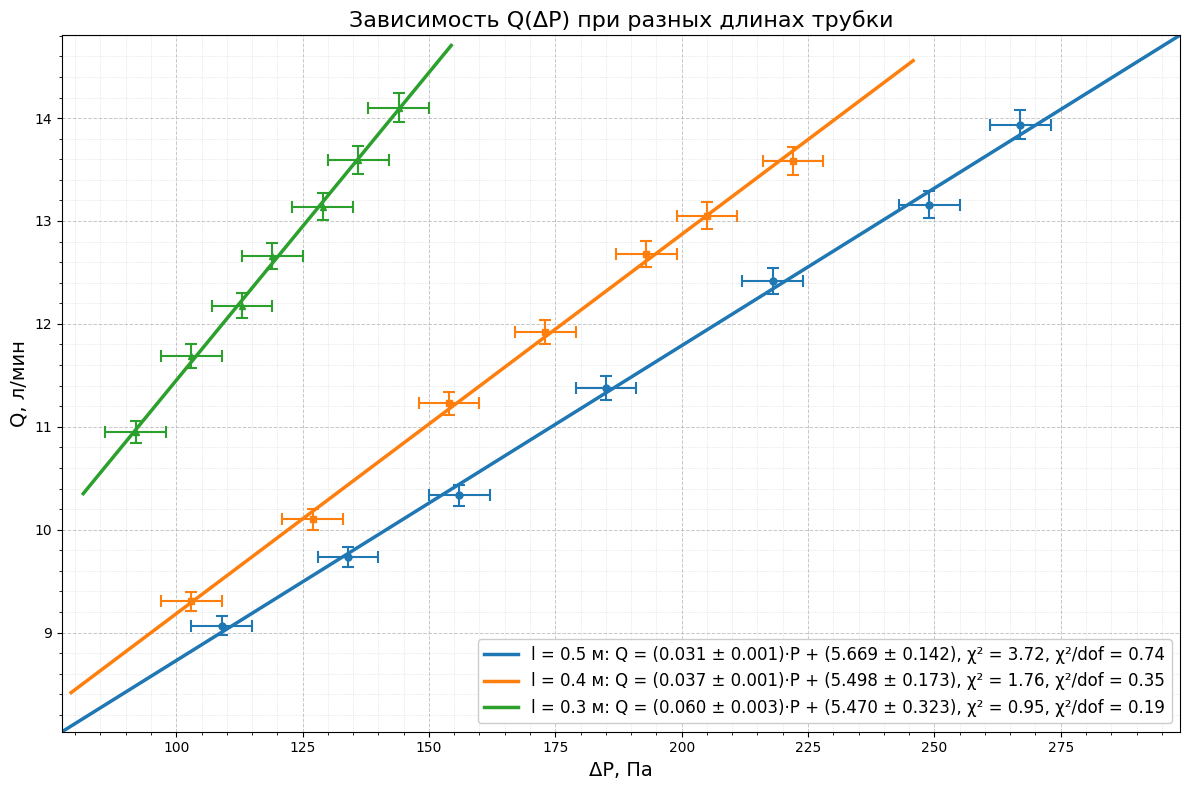
\includegraphics[width=0.95\textwidth]{graphs/turb2.png}}
    \caption[]{ Турбулентное течение, вторая трубка d = 5.25 \text{мм}}
    \end{figure}

    \begin{figure}[h!]
    \centering{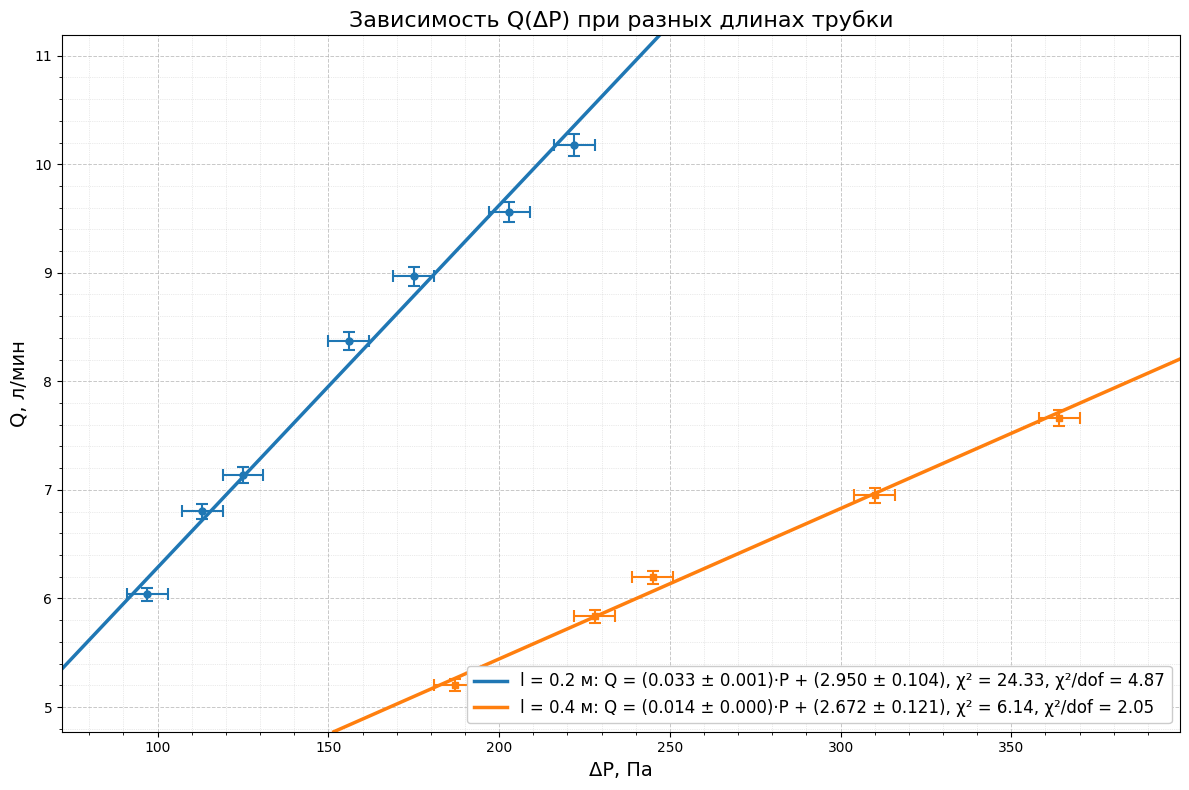
\includegraphics[width=0.95\textwidth]{graphs/turb3.png}}
    \caption[]{ Турбулентное течение, третья трубка d = 3.0 \text{мм}}
    \end{figure}
    



\end{document}


